% !TEX TS-program = pdflatex
% !TEX encoding = UTF-8 Unicode

\documentclass[11pt]{article} % use larger type; default would be 10pt

\usepackage[utf8]{inputenc} % set input encoding (not needed with XeLaTeX)

%%% PAGE DIMENSIONS
\usepackage[top=0.6in, left=0.8in, right=0.8in, bottom=0.7in]{geometry} % to change the page dimensions
\geometry{a4paper} % or letterpaper (US) or a5paper or....
% \geometry{margins=2in} % for example, change the margins to 2 inches all round
% \geometry{landscape} % set up the page for landscape

\usepackage{graphicx} % support the \includegraphics command and options

\usepackage[parfill]{parskip} % Activate to begin paragraphs with an empty line rather than an indent

%%% PACKAGES
\usepackage{booktabs} % for much better looking tables
\usepackage{array} % for better arrays (eg matrices) in maths
%\usepackage{paralist} % very flexible & customisable lists (eg. enumerate/itemize, etc.)
\usepackage{verbatim} % adds environment for commenting out blocks of text & for better verbatim
\usepackage{subfig} % make it possible to include more than one captioned figure/table in a single float
\usepackage{mathtools} % for math environments like align
\usepackage{amssymb} % for symbols like \therefore

%%% OPTIONAL PACKAGES
%\usepackage{braket}

%%% HEADERS & FOOTERS
\usepackage{fancyhdr} % This should be set AFTER setting up the page geometry
\pagestyle{fancy} % options: empty , plain , fancy
\renewcommand{\headrulewidth}{0pt} % customise the layout...
\lhead{}\chead{}\rhead{}
\lfoot{}\cfoot{\thepage}\rfoot{}

%%% SECTION TITLE APPEARANCE
%\usepackage{sectsty}
%\allsectionsfont{\sffamily\mdseries\upshape} % (See the fntguide.pdf for font help)

%%% ToC (table of contents) APPEARANCE
%\usepackage[nottoc,notlof,notlot]{tocbibind} % Put the bibliography in the ToC
%\usepackage[titles,subfigure]{tocloft} % Alter the style of the Table of Contents
%\renewcommand{\cftsecfont}{\rmfamily\mdseries\upshape}
%\renewcommand{\cftsecpagefont}{\rmfamily\mdseries\upshape} % No bold!

%%% END Article customizations

\author{Josh Wainwright \\ UID:1079596}

\title{Week 9 Assessment}

\date{}

\begin{document}

\maketitle
%\tableofcontents
%\vspace{1cm}\hrule \vspace{1cm}
%\newpage
\section{Parameters}
\begin{itemize}
	\item Generalisation Hierarchy Levels: 2
	\item M:N Relationships: 2
	\item Symetric Recursive Relationship: $1:1$
	\item Multi-valued Attribute: 1
\end{itemize}

\section{Astronomical Objects}
This database describes the classification of a few astronomical objects,
namely stars, planets and asteroids. Each of these objects has some aspects in
common and so a generalisation hierarchy is used. Each type of object has a
mass and an average distance that it lies from earth.

Stars are a type of object. In addition to the object attributes, they have a
luminosity, as viewed from earth. They can also exist in a binary system where
a star orbits at most one other star. Each star is made up of a number of
elements; hydrogen, helium, etc; each of which has an atomic mass and number.

Planets exist in isolation, but contain information about their orbital
duration, an optional star that they orbit (this must exist in the star table)
and a list of constituents that they are made from.

Asteroids have an associated eccentricity of their orbit (how non-circular it
is) as well as a number of discoverers who were responsible for finding and
measuring it.

\section{Business Rules}
\label{sec:business_rules}

\begin{enumerate}
	\item All stars, planets and asteroids are astronomical objects, called
		objects.
	\item Stars can orbit zero or 1 other star.
	\item Stars are composed of many elements and each element can appear in
		many stars.
	\item Planets are composed of two or more elements.
	\item Planet classification is either ``rocky'' or ``gasseous''.
	\item Asteroids all have one or more discoverers. Each asteroid can have
		multiple discoverers, representing a group discovery, and each
		discoverer can have discovered many asteroids.
\end{enumerate}

% section business_rules (end)

\newpage
\section{High Level ERD}
\label{sec:high_level_erd}

\begin{figure}[h!]
	\centering
	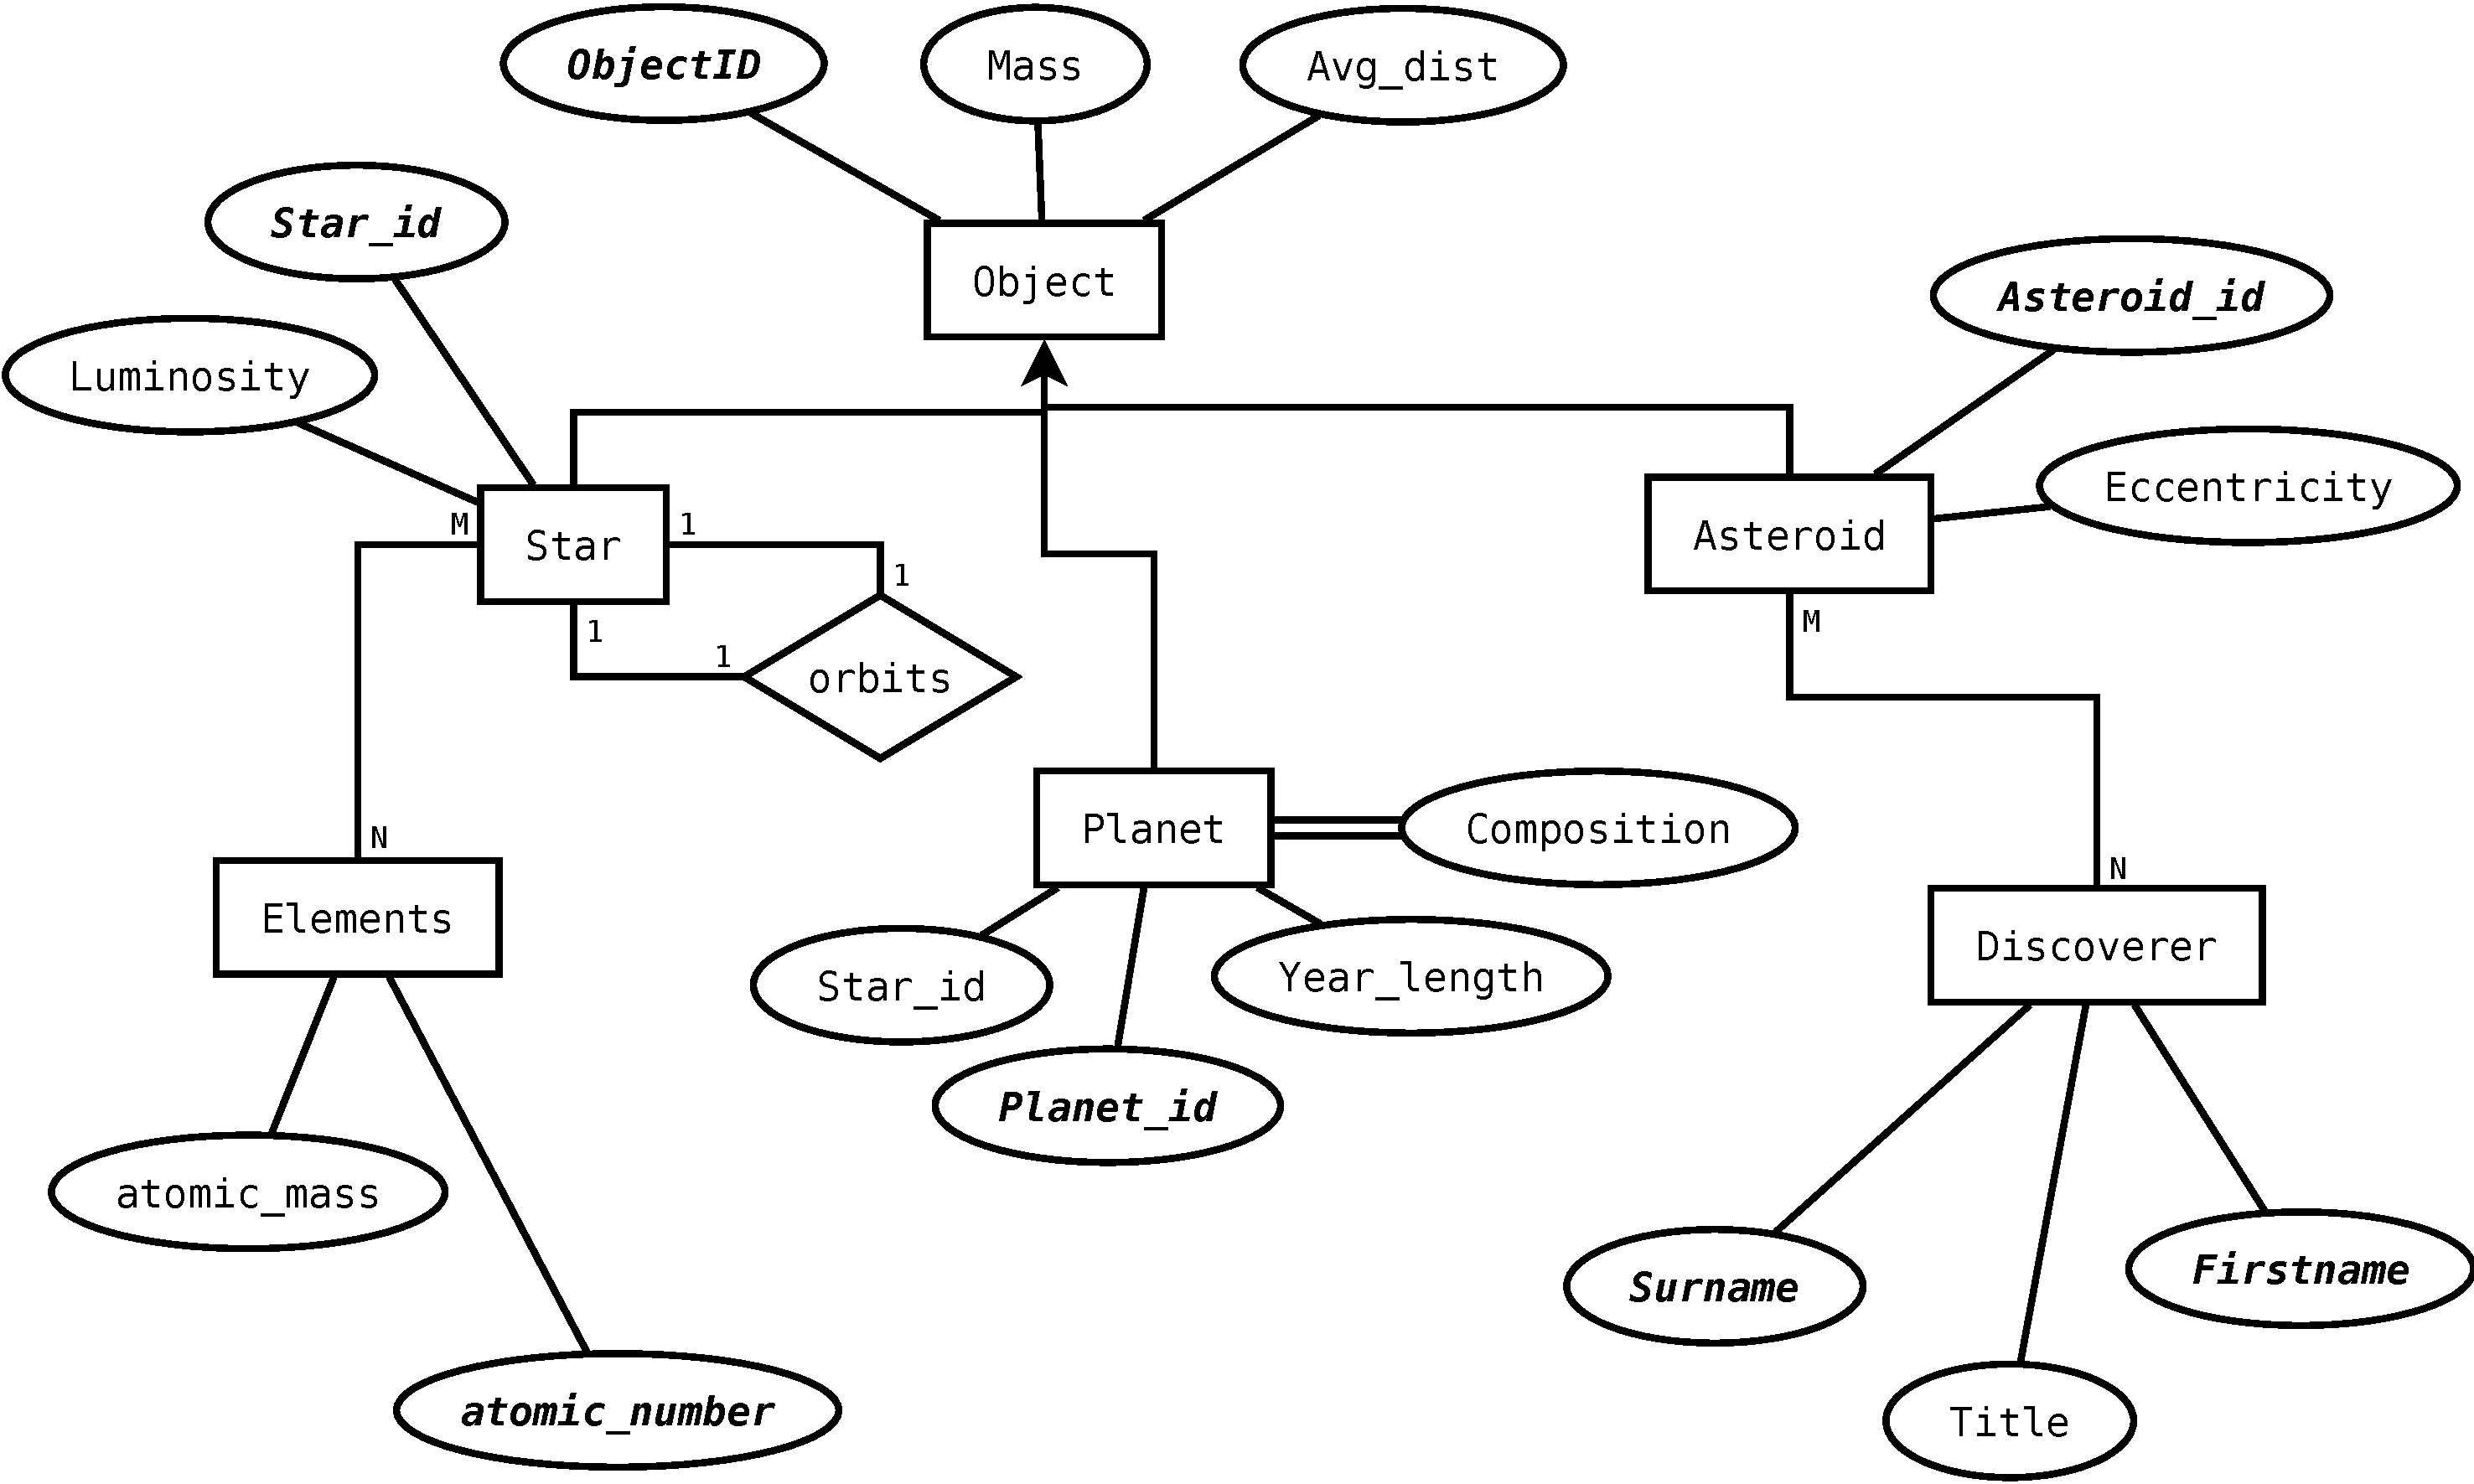
\includegraphics[width=1.0\textwidth]{ERD-high.pdf}
\end{figure}

\subsection{Notes}
\label{sub:notes}

\begin{itemize}
	\item Chen Entity Relationship Diagram.
	\item The attributes making up the primary key is shown in bold.
	\item All generalisation hierarchies have exhaustive relationships.
	\item A subtype to supertype relationship is denoted with an arrow from
		subtype to supertype.
	\item Multi-valued attributes are shown with a double line.
\end{itemize}

% subsection notes (end)

% section high_level_erd (end)

\newpage
\section{Low Level ERD}
\label{sec:low_level_erd}

\begin{figure}[h]
	\centering
	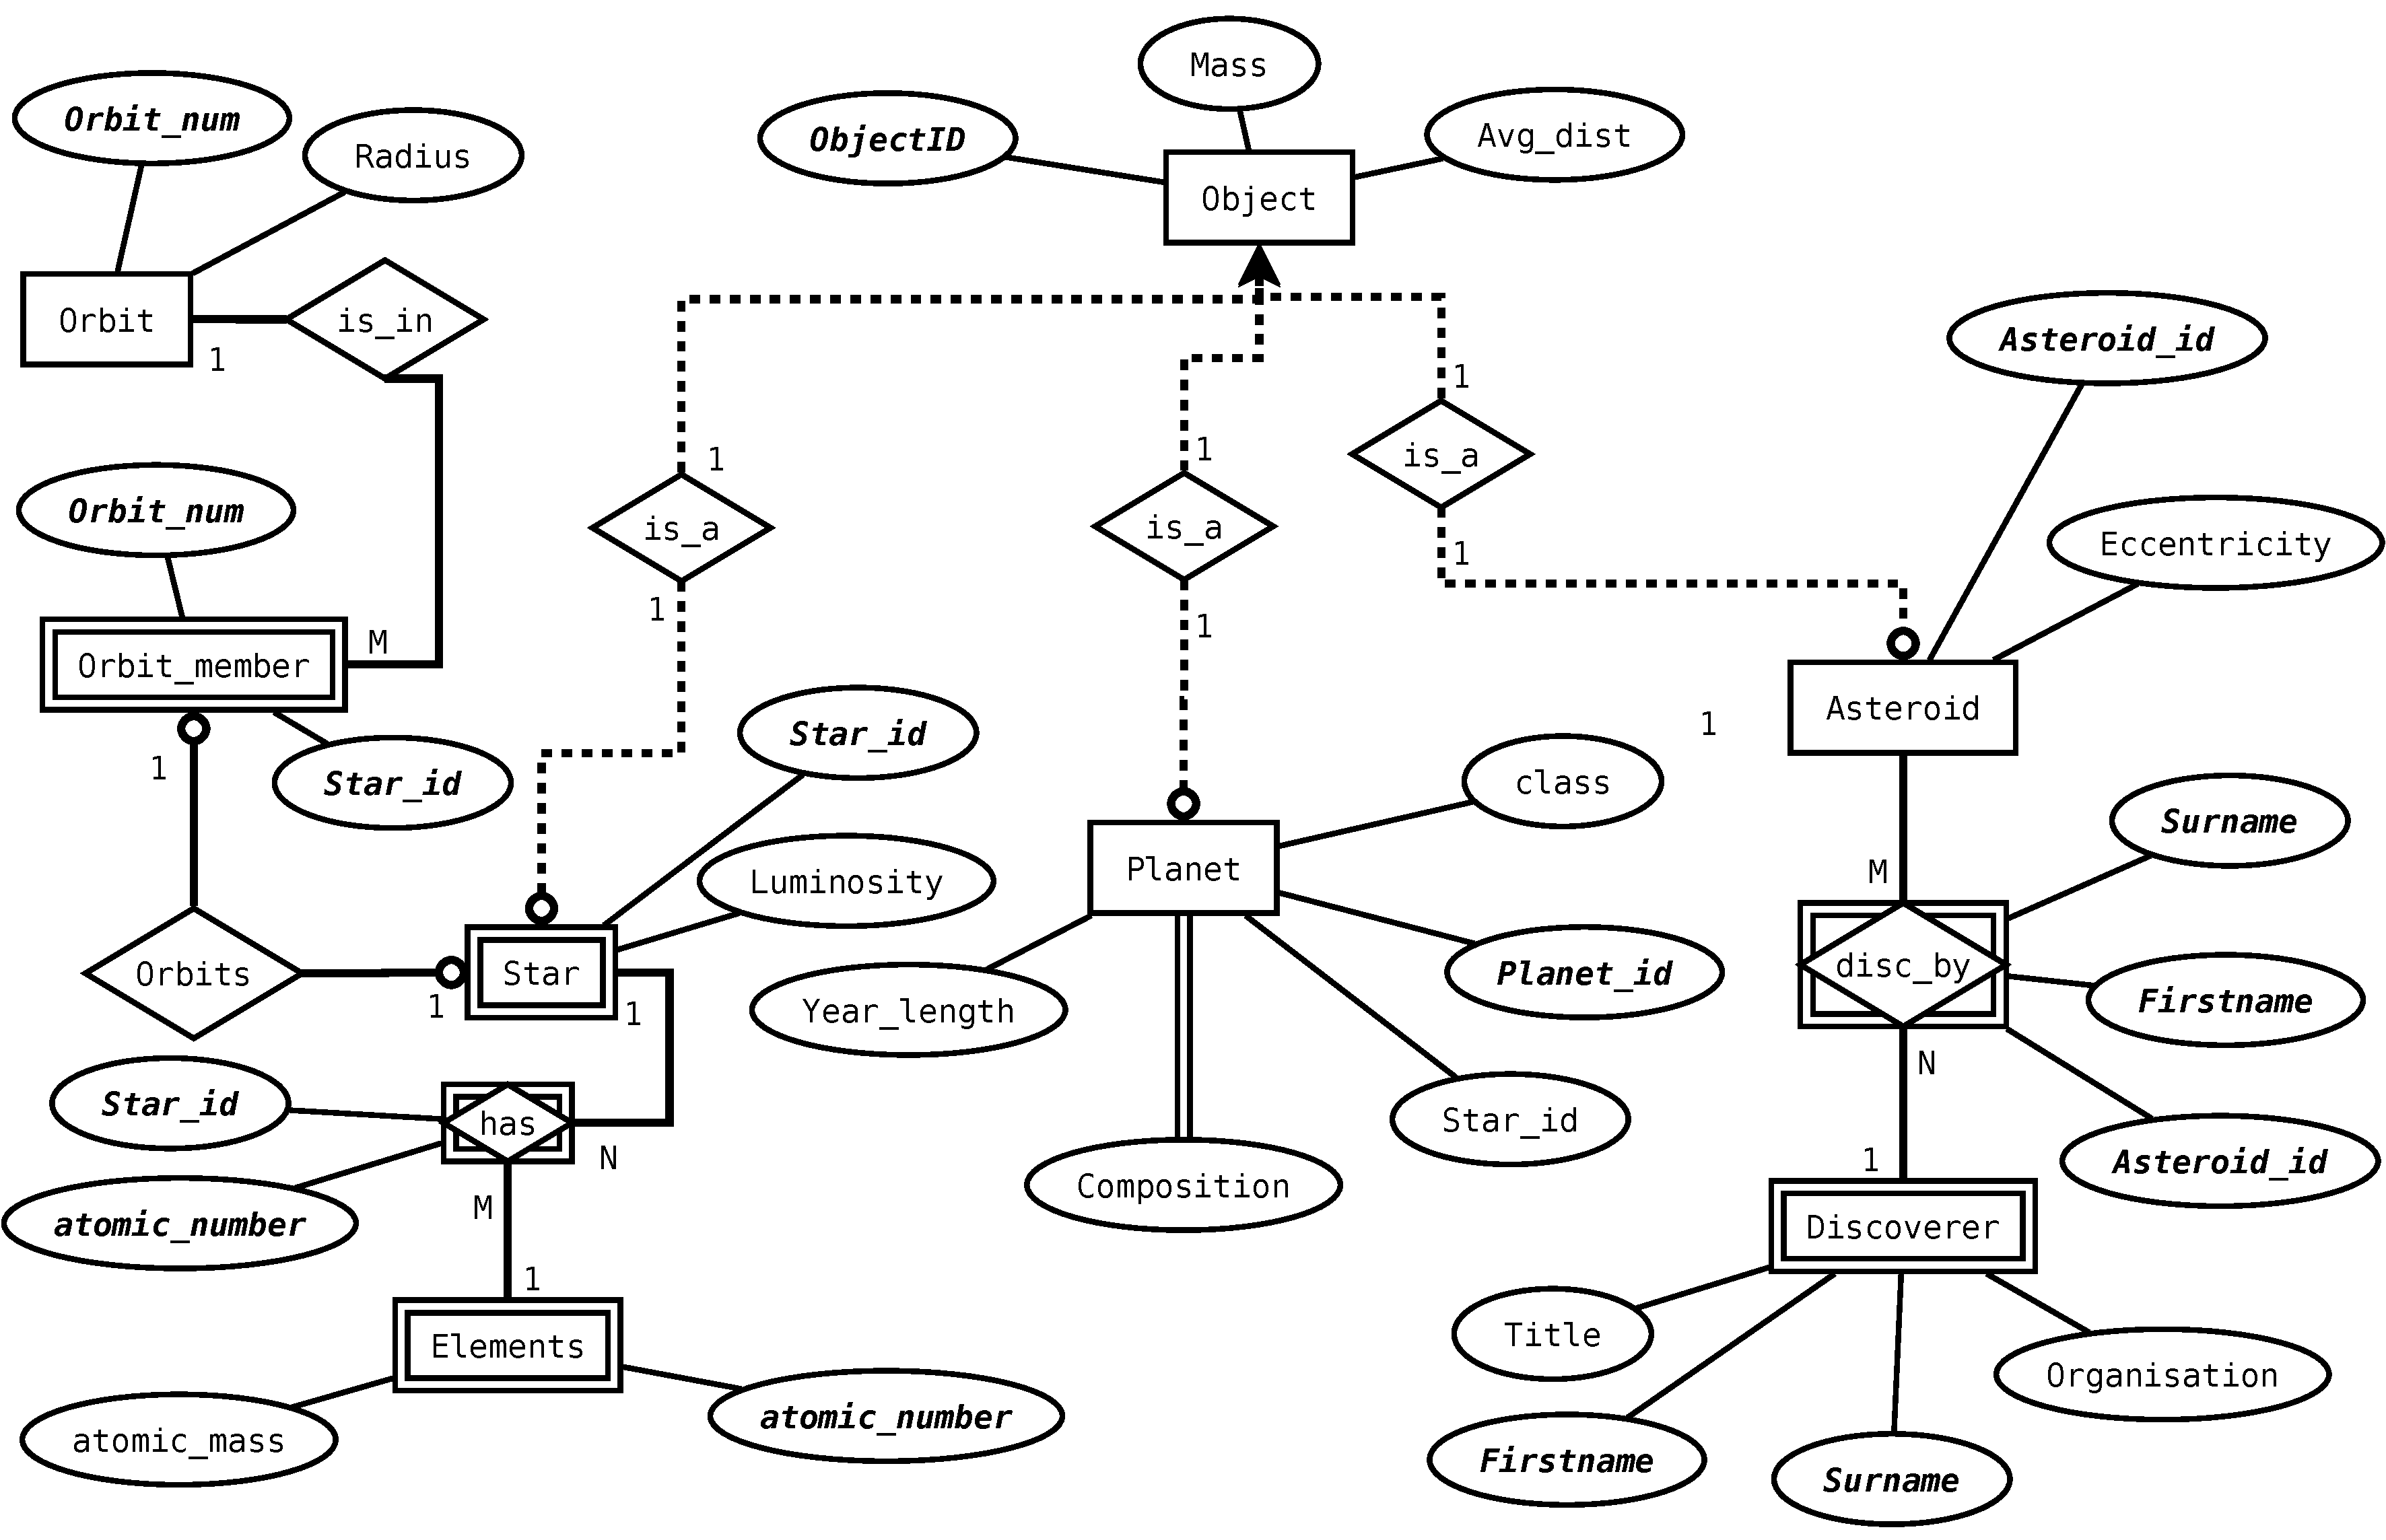
\includegraphics[width=1.0\textwidth]{ERD-low-Chen.pdf}
\end{figure}

\subsection{Notes}
\label{sub:notes}

\begin{itemize}
	\item Chen Entity Relationship Diagram.
	\item Attributes making up the primary key are shown in bold.
	\item Recursive relationships have been broken down.
	\item Weak relationships are shown with a dotted line, strong with a bold
		line.
	\item Weak entity types have a double border.
	\item Mulivalued attributes have been split into separate tables.
\end{itemize}

% subsection notes (end)

% section low_level_erd (end)

\newpage
\section{Low Level ERD}
\label{sec:low_level_erd}

\begin{figure}[h]
	\centering
	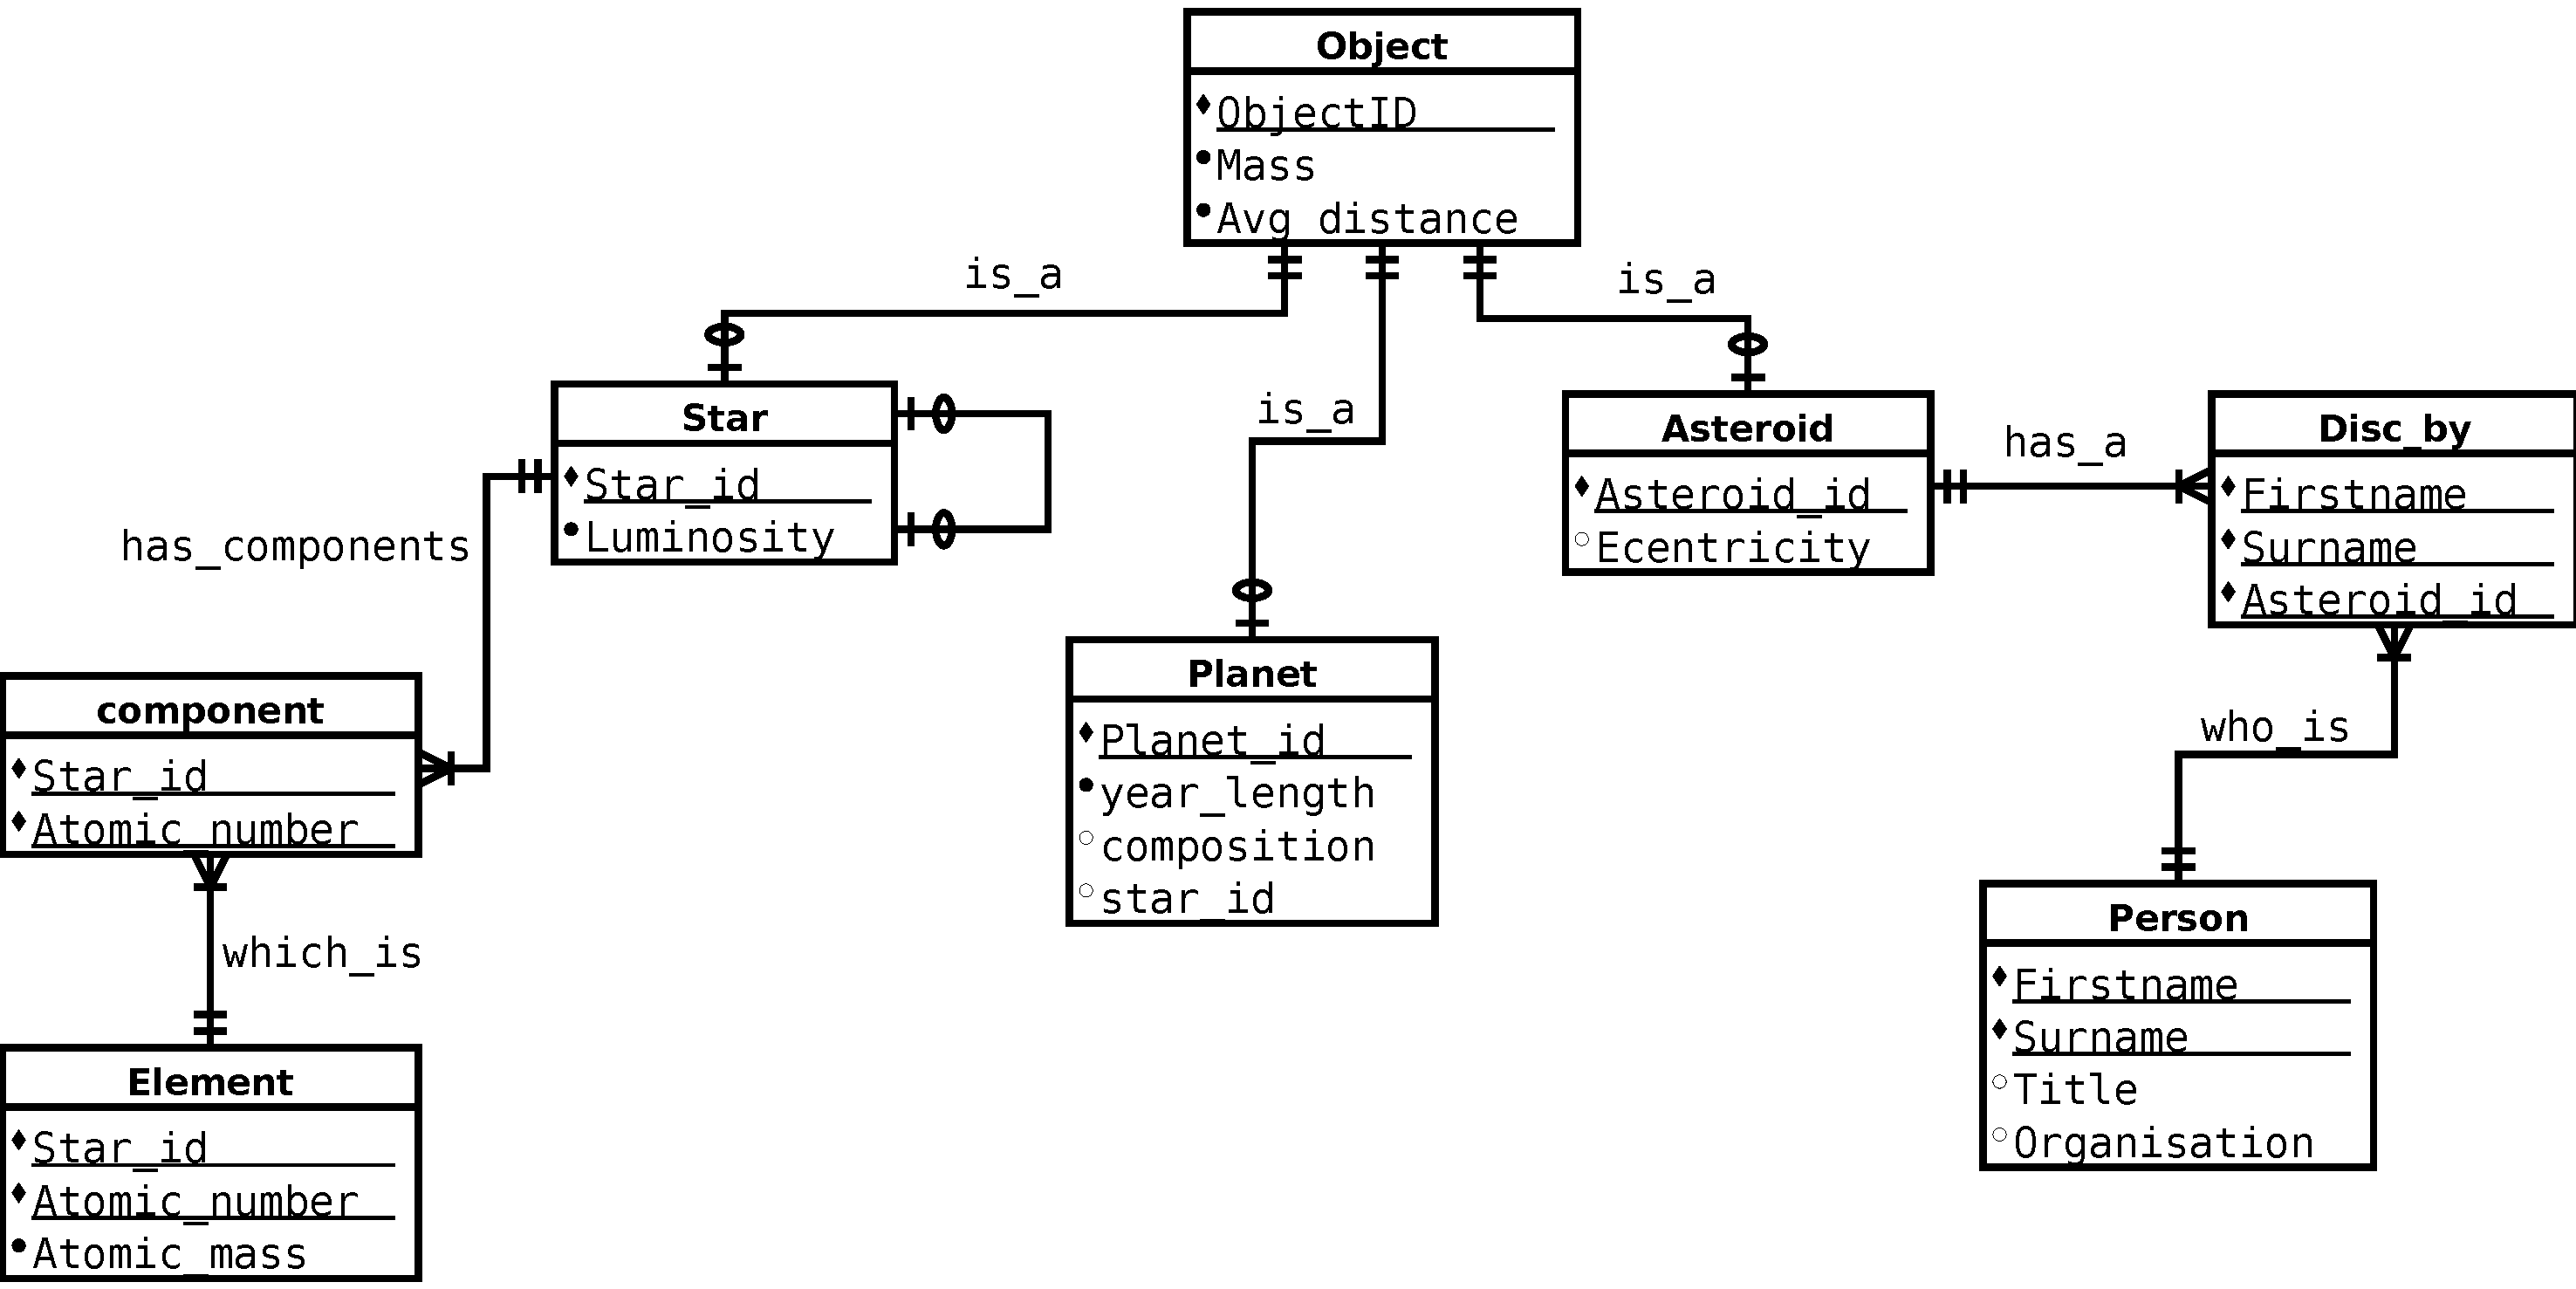
\includegraphics[width=1.0\textwidth]{ERD-low-CF.pdf}
\end{figure}

% section low_level_erd (end)

\end{document}
